% generated by scripts/pkl_to_latex.py
% source PKL : tscan_v1_L8_Ne8_U10_mode-uniform_nmin2_solver-gcg_full_restarts4_iter200_kmax4_tol1em09_t0.05to2_N20-d03538a42051.pkl
% scan type  : tscan
% state      : gs
% requires   : \usepackage{pgfplots} \pgfplotsset{compat=1.18}
% colours match the matplotlib PDF (tab10 cycle)
\definecolor{gmeC0}{HTML}{1F77B4}
\definecolor{gmeC1}{HTML}{FF7F0E}
\definecolor{gmeC2}{HTML}{2CA02C}
\definecolor{gmeC3}{HTML}{D62728}
\definecolor{gmeC4}{HTML}{9467BD}
\definecolor{gmeC5}{HTML}{8C564B}
\definecolor{gmeC6}{HTML}{E377C2}
\definecolor{gmeC7}{HTML}{17BECF}

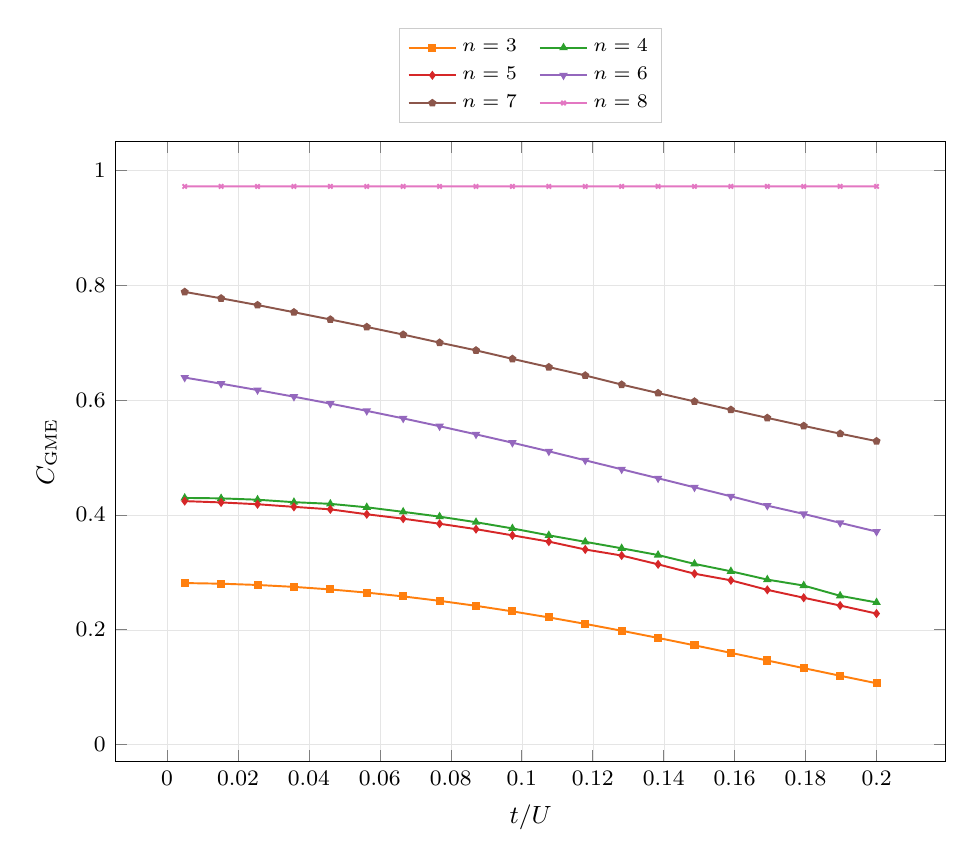
\begin{tikzpicture}
  \begin{axis}[
    width=\columnwidth,
    height=0.78\columnwidth,
    xlabel={$t/U$},
    ylabel={$C_{\mathrm{GME}}$},
    grid=both,
    grid style={line width=.1pt, draw=gray!20},
    tick label style={font=\footnotesize\rmfamily, /pgf/number format/fixed},
    label style={font=\small\rmfamily},
    scaled ticks=false,
    legend style={font=\scriptsize\rmfamily, draw=gray!40, at={(0.5,1.03)}, anchor=south, /tikz/every even column/.append style={column sep=6pt}},
    legend cell align={left},
    legend columns=2,
    ymin=-0.03,
    ymax=1.05,
  ]
    \addplot[color=gmeC1, mark=square*, mark size=1.1pt, line width=0.7pt] coordinates {
        (0.005,0.281155) (0.015263,0.280054) (0.025526,0.277837) (0.035789,0.274506)
        (0.046053,0.270066) (0.056316,0.264526) (0.066579,0.2579) (0.076842,0.250218)
        (0.087105,0.241521) (0.097368,0.231872) (0.107632,0.22135) (0.117895,0.210057)
        (0.128158,0.198107) (0.138421,0.185627) (0.148684,0.17275) (0.158947,0.159605)
        (0.169211,0.146318) (0.179474,0.133001) (0.189737,0.119754) (0.2,0.106664)
    };
    \addlegendentry{$n=3$}
    \addplot[color=gmeC2, mark=triangle*, mark size=1.1pt, line width=0.7pt] coordinates {
        (0.005,0.429405) (0.015263,0.428677) (0.025526,0.426283) (0.035789,0.422004)
        (0.046053,0.4191) (0.056316,0.413075) (0.066579,0.405177) (0.076842,0.396825)
        (0.087105,0.387122) (0.097368,0.376285) (0.107632,0.364262) (0.117895,0.352968)
        (0.128158,0.341686) (0.138421,0.329965) (0.148684,0.314528) (0.158947,0.301658)
        (0.169211,0.287186) (0.179474,0.276798) (0.189737,0.258977) (0.2,0.247387)
    };
    \addlegendentry{$n=4$}
    \addplot[color=gmeC3, mark=diamond*, mark size=1.1pt, line width=0.7pt] coordinates {
        (0.005,0.423856) (0.015263,0.421572) (0.025526,0.41842) (0.035789,0.41386)
        (0.046053,0.409542) (0.056316,0.400951) (0.066579,0.393286) (0.076842,0.384452)
        (0.087105,0.375033) (0.097368,0.364277) (0.107632,0.35332) (0.117895,0.339626)
        (0.128158,0.329095) (0.138421,0.313766) (0.148684,0.297462) (0.158947,0.285934)
        (0.169211,0.269349) (0.179474,0.255586) (0.189737,0.242) (0.2,0.228007)
    };
    \addlegendentry{$n=5$}
    \addplot[color=gmeC4, mark=triangle*, mark size=1.1pt, mark options={rotate=180}, line width=0.7pt] coordinates {
        (0.005,0.639041) (0.015263,0.628374) (0.025526,0.617268) (0.035789,0.605717)
        (0.046053,0.593634) (0.056316,0.58105) (0.066579,0.567947) (0.076842,0.554302)
        (0.087105,0.540123) (0.097368,0.525558) (0.107632,0.510531) (0.117895,0.494931)
        (0.128158,0.479274) (0.138421,0.463624) (0.148684,0.447914) (0.158947,0.432283)
        (0.169211,0.415984) (0.179474,0.401563) (0.189737,0.386055) (0.2,0.370771)
    };
    \addlegendentry{$n=6$}
    \addplot[color=gmeC5, mark=pentagon*, mark size=1.1pt, line width=0.7pt] coordinates {
        (0.005,0.788202) (0.015263,0.777014) (0.025526,0.765277) (0.035789,0.752792)
        (0.046053,0.740171) (0.056316,0.727184) (0.066579,0.713864) (0.076842,0.699867)
        (0.087105,0.686387) (0.097368,0.671611) (0.107632,0.657214) (0.117895,0.642723)
        (0.128158,0.626781) (0.138421,0.612037) (0.148684,0.597411) (0.158947,0.582975)
        (0.169211,0.568785) (0.179474,0.554906) (0.189737,0.541323) (0.2,0.528287)
    };
    \addlegendentry{$n=7$}
    \addplot[color=gmeC6, mark=x, mark size=1.1pt, line width=0.7pt] coordinates {
        (0.005,0.971886) (0.015263,0.971886) (0.025526,0.971886) (0.035789,0.971886)
        (0.046053,0.971887) (0.056316,0.971887) (0.066579,0.971887) (0.076842,0.971888)
        (0.087105,0.971888) (0.097368,0.97189) (0.107632,0.971891) (0.117895,0.971892)
        (0.128158,0.971894) (0.138421,0.971897) (0.148684,0.9719) (0.158947,0.971903)
        (0.169211,0.971906) (0.179474,0.97191) (0.189737,0.971914) (0.2,0.971918)
    };
    \addlegendentry{$n=8$}
  \end{axis}
\end{tikzpicture}
